\section{Technické vybavení akvária}
    V této kapitole je uveden výčet základní akvaristické techniky nutné k provozu domácího akvária, rozčleněné podle svého účelu. Ve druhé části se text věnuje přehledu různých dostupných komplexních systémů zaměřujících se na automatizaci provozu akvária. Cílem kapitoly je seznámit čtenáře blíže s problematikou založení a provozu akvária a různými možnostmi technického zajištění jak domácích, tak i profesionálních akvárií.
    \subsection{Filtrace vody}
        Úkolem filtru je průběžně odstraňovat z vody nečistoty a to jak mechanické, tak zejména v podobě škodlivých látek vznikajících v akváriu. Filtrační materiál je volen tak, aby tvořil vhodné prostředí pro život filtračních bakterií, které se těmito škodlivými látkami živí \cite{yt-filtrace}. Rozlišujeme tři základní typy akvarijních filtrů -- vnější, vnitřní a závěsné. Na obr.~\ref{fig:filtry-srovnani} se nachází ukázka vybraných zástupců jednotlivých typů.
        
        \textbf{Vnějším filtrem} se rozumí zařízení umístěné obvykle ve skříňce pod akváriem, mívá připojeny dvě hadice -- na vstup a výstup vody. Toto řešení je považováno za nejlepší, protože filtr není omezen rozměry a může tak dosahovat daleko vyššího výkonu a účinnější filtrace díky většímu množství filtračních materiálů. 

        \textbf{Vnitřní filtr} (někdy také ponorný) je levným, ale nepříliš účinným řešením pro malá akvária. Nachází se z velké částo v akváriu a za pomocí motorku tlačí vodu přes obvykle molitanovou náplň.

        \textbf{Závěsný filtr}  je kompromisním řešením.  Cenou i účinností filtrace se pohybuje mezi oběma zmíněnými typy. Nezabírá prostor uvnitř akvária a může tak využít větší objem filtrační hmoty než filtr vnitřní. Instalace je provedena zavěšením na stěnu akvária, je tedy velmi jednoduchá. 

        \begin{figure}[h!]
            \centering
            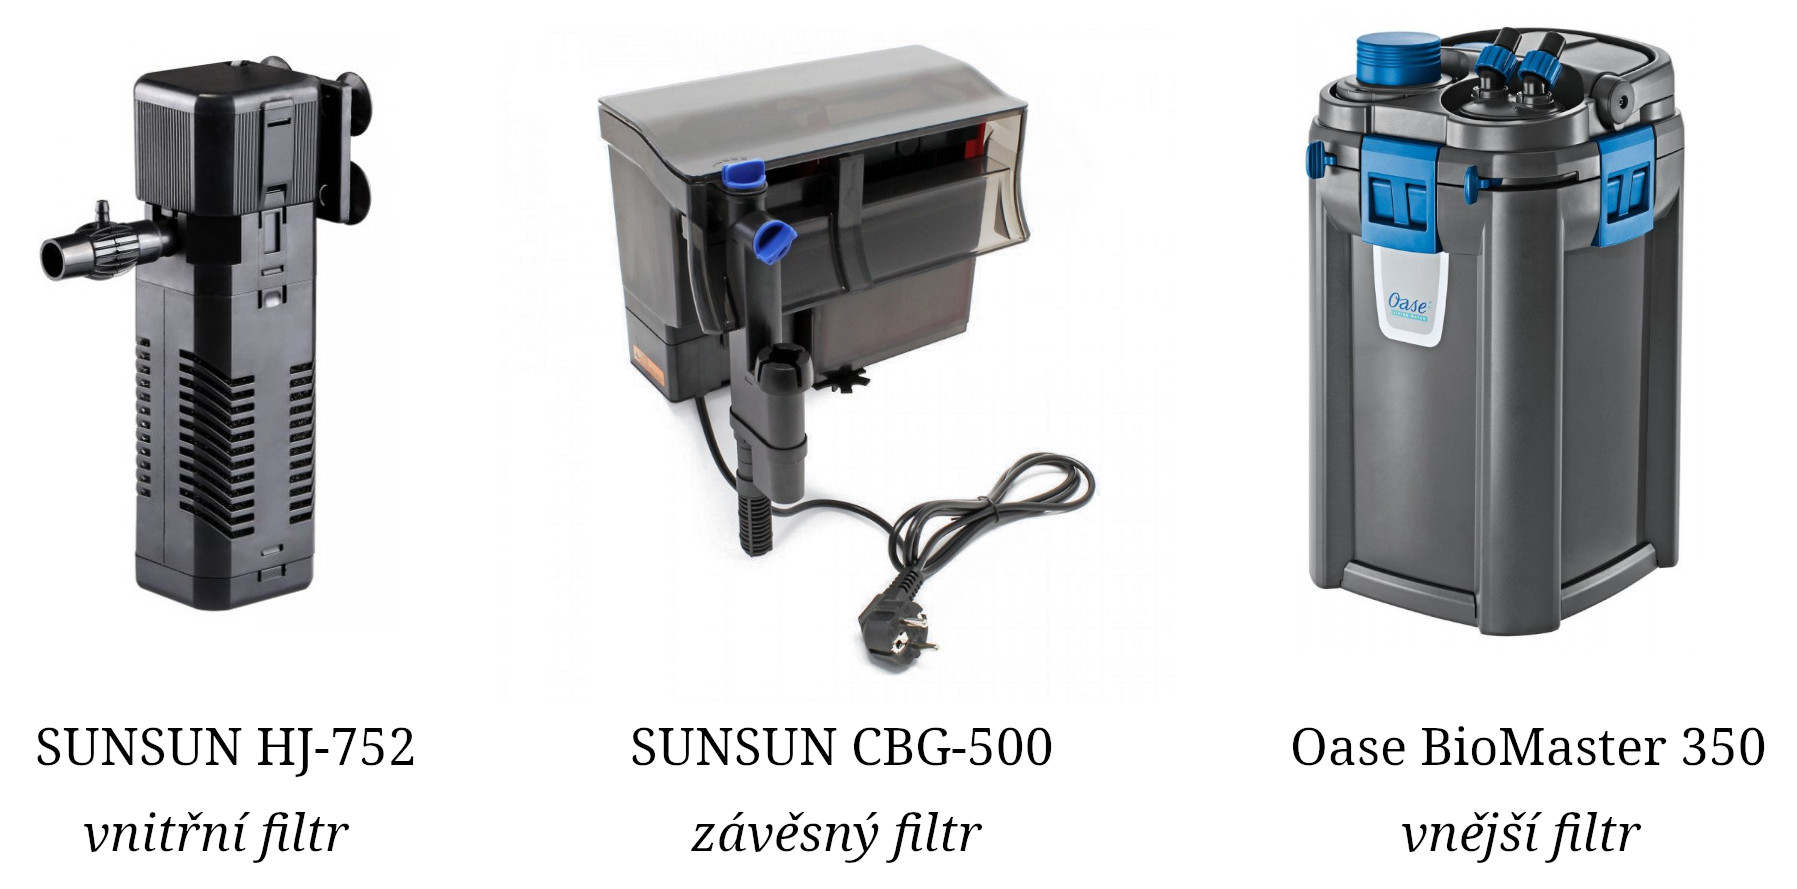
\includegraphics[width=\textwidth]{obrazky/filtry/filtry.jpg}
            \caption{Příklad různých typů filtrů. Fotografie převzaty z \cite{eshop-rostlinna-akvaria}}
            \label{fig:filtry-srovnani}
        \end{figure}

    \subsection{Osvětlení}
        Funkce osvětlení akvária je dvojí. Jednak jde o estetický dojem z pohledu pozorovatele, kdy vhodné nasvícení přidává akváriu na atraktivitě. Druhak se osvětlení snaží nasimulovat osazenstvu akvária přirozené životní podmínky, aby celý ekosystém mohl fungovat.

        Hlavními parametry při výběru svítidla je jeho \textbf{intenzita}, \textbf{spektální charakteristika} a \textbf{spotřeba}. 
        
        Příliš intenzivní světlo zvyšuje riziko nežádoucí tvorby řas a pro ryby může být stresovým faktorem, nízká intenzita zase může způsobit špatný růst rostlin~\cite{KejzlarRadim2022Ařpa}. Na internetu existuje mnoho návodů a rad na stanovení správné intenzity, ale protože zde hraje roli spousta dalších parametrů jako např. výška hladiny nebo konkrétní typ rostlin, je vhodné tyto hodnoty brát pouze jako orientační a intenzitu osvětlení upravit během provozu podle potřeby. Výpočet se také liší pro jednotlivé typy svítidel. 

        Spektrum světla hraje roli hned z několika důvodů. Rostliny pro tvorbu chlorofylu a následnou fotosyntézu potřebují světlo zejména vlnových délek \qty{440}{nm} (modrá barva) a \qty{660}{nm} (červená barva)~\cite{eshop-ledsolution-svetlo}, pokud by zvolené osvětlení tyto vlnové délky neobsahovalo, nemohou rostliny správně fungovat. Akvárium osvětlené pouze těmito dvěma barvami by ale nevypadalo vizuálně dobře, proto se využívá také širokospektrální bílé světlo, které svým spektrem odpovídá co nejlépe dennímu světlu. 
        Specializovaná svítidla pak nabízejí možnost napodobit světelné spektrum různých vodních prostředí a přizpůsobit se tak i rostlinám a živočichům žijícím ve velkých hloubkách. 

 
        \begin{figure}[h!]
            \centering
            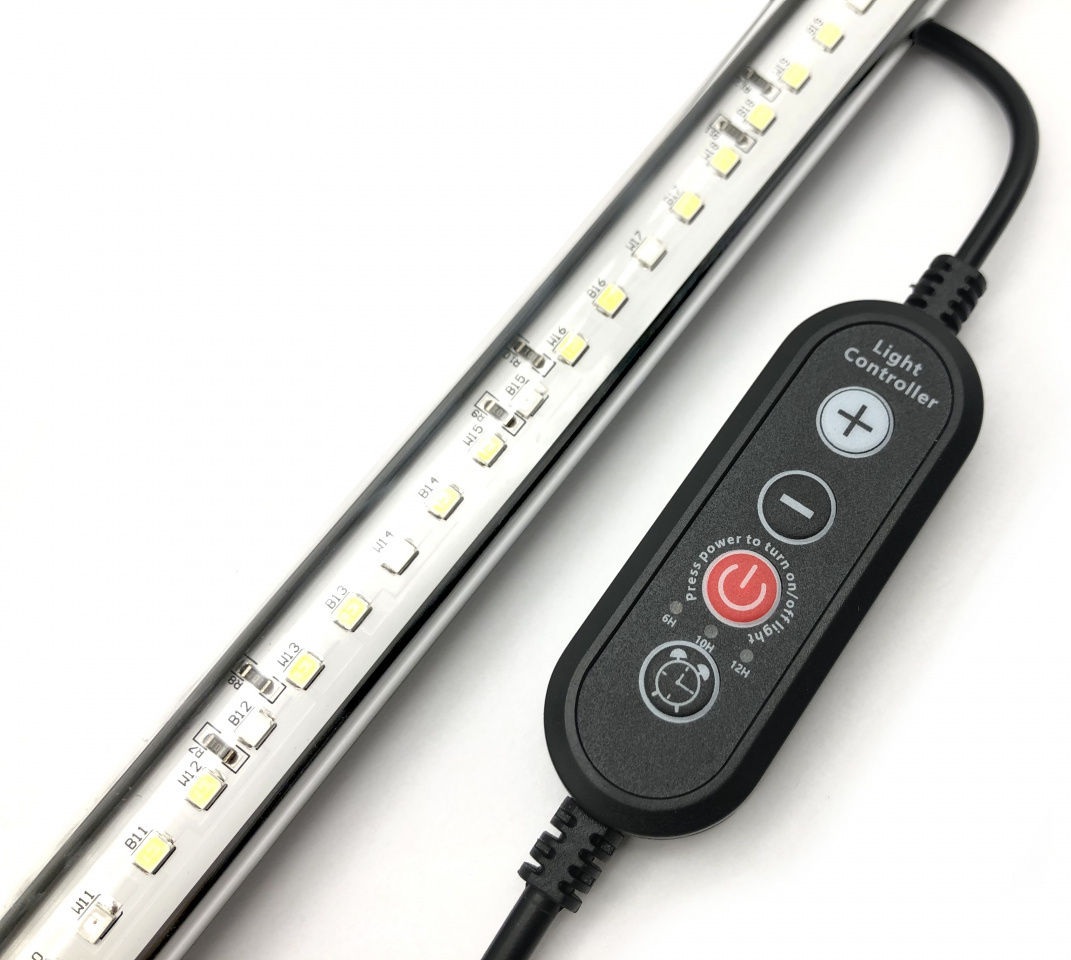
\includegraphics[width=0.6\textwidth]{obrazky/osvetleni/stmivac.jpg}
            \caption{Trubice s LED páskem a manuální stmívač a časovač. Převzato z~\cite{eshop-rostlinna-akvaria}.}
            \label{fig:obrazky-osvetleni-stmivac-jpg}
        \end{figure}

        Na trhu jsou v současné době tři typy akvaristických světel: \textbf{zářivky}, \textbf{výbojky}  a \textbf{LED svítidla}~\cite{eshop-rostlinna-akvaria-svetlo}. Zářivky jsou považovány za dnes již nepříliš moderní řešení a bývají nahrazovány LED svítidly, ty se vyznačují lepší účinností (tedy nižší spotřebou energie při stejné intenzitě světla), delší životností a širší paletou barev. U zářivek také nebylo možné plynule regulovat intenzitu, jako je tomu u LED, a dosáhnout tak např. postupného rozsvícení nebo zhasnutí světla simulujícího východ a západ slunce. Skoková změna při zapnutí nebo vypnutí světla je pro ryby také zbytečným stresovým faktorem~\cite{MusilLibor2018Isps}. Co se týče výbojek, ty nacházejí uplatňení zejména pro hluboké nádrže, protože jejich světlo je bodové a intenzita dostačující k prosvícení velkého objemu vody, spotřeba energie je ale v porovnání s LED vysoká, takže pokud to není nezbytně nutné, je lepší se jim vyhnout.   

        Typické domácí akvárium je osvětleno jedním nebo několika samostatně stmivatelnými LED svítidly a to buďto v podobě LED pásků nalepených na hliníkovém profilu anebo hotového svítidla, ve kterém jsou čipy s LED zabudovány napevno. Stmívání je nastavováno buď ručně anebo za pomoci mobilní aplikace dodané výrobcem stmívače. Příklad běžně dostupného výrobku lze vidět na obr.~\ref{fig:obrazky-osvetleni-stmivac-jpg}.

    \subsection{Ohřev}
        Většina okrasných sladkovodních ryb běžně chovaných akvaristy pochází z tropických krajů a vyžaduje teplotu vody v rozmezí 22 -- \qty{26}{\degreeCelsius}~\cite{slavotinek2014}, to je o něco málo vyšší teplota než bývá v domácnosti typická a proto je nutné zajistit akváriu možnost dodatečného ohřevu. Nejčastějsím řešením je ponorné topné těleso na odporové bázi s vlastní termostatovou regulací, viz obr.~\ref{fig:obrazky-topeni-topitko-jpg}.

        \begin{figure}[h!]
            \centering
            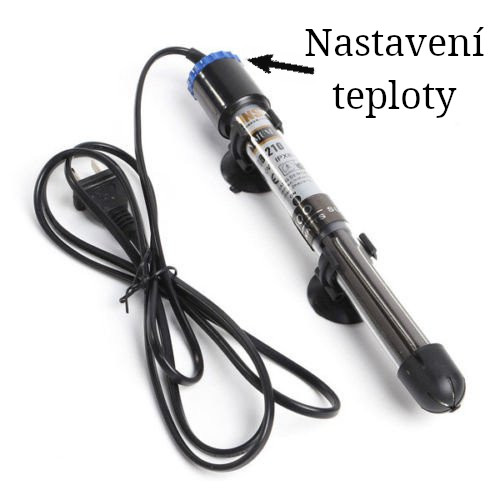
\includegraphics[width=0.7\textwidth]{obrazky/topeni/topitko.jpg}
            \caption{SUNSUN topítko 100W s termostatem. Převzato z \cite{eshop-rostlinna-akvaria}.}
            \label{fig:obrazky-topeni-topitko-jpg}
        \end{figure}
        
        Z principu fungování termostatu vyplývá, že výsledná teplota vody není v čase konstantní, ale osciluje okolo nastavené hodnoty. Rozsah kolísání teploty je pak závislý na hysterezi termostatu, obecně lze říci, že to může být i několik stupňů. Pro většinu aplikací to není velký problém, ale některé druhy ryb mohou být na změny teploty náchylnější, v takovém případě je potřeba buďto vybrat topítko takové, kde výrobce rozsah teplot uvádí, anebo zvolit jiný způsob regulace. 

    \subsection{Monitorování}
        Jak již vyplynulo z úvodních kapitol, v akváriu probíhá celá řada procesů ovlivňujících jeho stav. Klíčem k vytvoření prosperujícího akvária je dosažení rovnováhy a stability mezi nimi za pomoci vhodně nastavené akvarijní techniky. Nejen u začínajících akvaristů se mohou vyskytnout problémy s růstem rostlin, zdravím ryb nebo třeba výskytem řasy. Odhalit příčiny těchto problémů může být mnohdy obtížné, ovzláště pokud není k dispozici dostatečné množství informací o tom, co se v akváriu děje. 
        
        Existuje několik veličin, které úzce souvisí s procesy v akváriu a které je možné také poměrně jednoduše sledovat. Na trhu je celá řada produktů sloužících k tomuto účelu. Většinou je na výběr možnost analogového nebo čistě mechanického přístroje případně samostatného digitálního čidla, existují však také komplexní řešení, těm se dále věnuje kapitola  \ref{lab:kapitola-komplexni-reseni}. 

        \subsubsection{Teplota}
            Umístěním teploměru (ať už v analogové nebo digitální podobě) do akvária je možné zkontrolovat správné nastavení topného tělesa a následně provést jeho úpravu. Také lze včas získat informaci o jeho případné poruše a nebo třeba jen nedostatečném výkonu. 
        \subsubsection{pH a CO\(\mathbf{_{2}}\)}
            Hodnota pH popisuje kyselost resp. zásaditost měřeného vodného roztoku. Běžně se používá logaritmická stupnice s hodnotami 0 až 14, přičemž zcela neutrální voda má pH rovno 7, menší hodnoty mají roztoky kyselé a větší než 7 pak roztoky zásadité.  Obecně lze říci, že pro ryby je vyhovující pH v rozsahu 6 až 8~\cite{slavotinek2014}. 

            Důležitým parametrem vody z pohledu rostlin a ryb je koncentrace \acs{co2}. Přirozeně platí, že rostliny \acs{co2} spotřebovávají při fotosyntéze a jistá koncentrace je tedy nutná pro jejich prosperitu, naopak příliš vysoká koncentrace může být nebezpečná pro ryby, kterým (obdobně jako např. lidem) komplikuje dýchání. Obsah \acs{co2} ve vodě je obtížné přímo měřit, jeho měnící se koncentrace má ale vliv právě na hodnoty pH, s rostoucí koncentrací \acs{co2} se pH vody snižuje a obráceně~\cite{DvorakJan2014RPpa,KejzlarRadim2022Ařpa}. 

            K měření pH vody se používají různé chemické testy (kapkové testy, testovací papírky), které je možné zakoupit v chovatelských potřebách. Z pohledu automatizace je mnohem zajímavějším řešením pH sonda, která umožňuje nepřetržité měření této veličiny a případnou okamžitou regulaci dávkování \acs{co2}.

             
    \subsection{Dostupná komplexní řešení}
    \label{lab:kapitola-komplexni-reseni}
        Tato sekce se věnuje porovnání několika nejznámějších systémů v oblasti automatizace akvárií. Je důležité připomenout, že ve všech oblastech elektrotechniky dochází k rychlému rozvoji a každý rok se na trhu objevují nové produkty se stále lepšími parametry a nižší cenou. Informace uvedené v této kapitole, a to zejména cenové údaje, se mohou velmi rychle stát neaktuálními a jsou tedy relevantní pouze v době vzniku této práce.

        Při tvorbě této kapitoly byly jako zdroj informací použity jednak oficiální materiály výrobců, ty ovšem samozřejmě obsahují vždy pouze pozitivní informace, dále pak různé uživatelské recenze na platformě YouTube popř. diskuzních fórech, nejedná se o zcela seriózní zdroje a proto je nutné také informace z této kapitoly brát s rezervou. 

        \subsubsection{GHL -- ProfiLux}
            Německá firma GHL se v oblasti akvaristiky pohybuje již přes 20 let a patří nepochybně ke špičce na trhu z hlediska komplexity a spolehlivosti. Základem jejich systému ProfiLux je kontrolér (např. nejmenší varianta viz obr.~\ref{fig:obrazky-trh-GHL-ProfiLux-Mini-jpg}), který je možné konfigurovat z PC za pomocí kabelu anebo vzdáleně s použitím aplikace nebo webového rozhraní. Ke kontroleru lze připojit celou řadu periferíí z portfolia firmy, jedná se o různé typy senzorů, dávkovače (pro úpravu parametrů vody), pumpy nebo řiditelný prodlužovací přívod pro síťové zásuvky (laicky řečeno \uv{chytrá prodlužovačka}). Společnost si zakládá na opravdu vysoké kvalitě a přesnosti svých výrobků, což se ale odráží také na jejich ceně. 

            Na výběr je z několika variant systému, přičemž ty nejdražší dokážou obsloužit i opravdu rozsáhlé a náročné akvaristické instalace. Cena nejlevnějšího základního setu je přibližně od \qty{10000}{Kč}~\cite{ghl-profilux,eshop-ghl-profilux-sets}.

            \begin{figure}[h!]
                \centering
                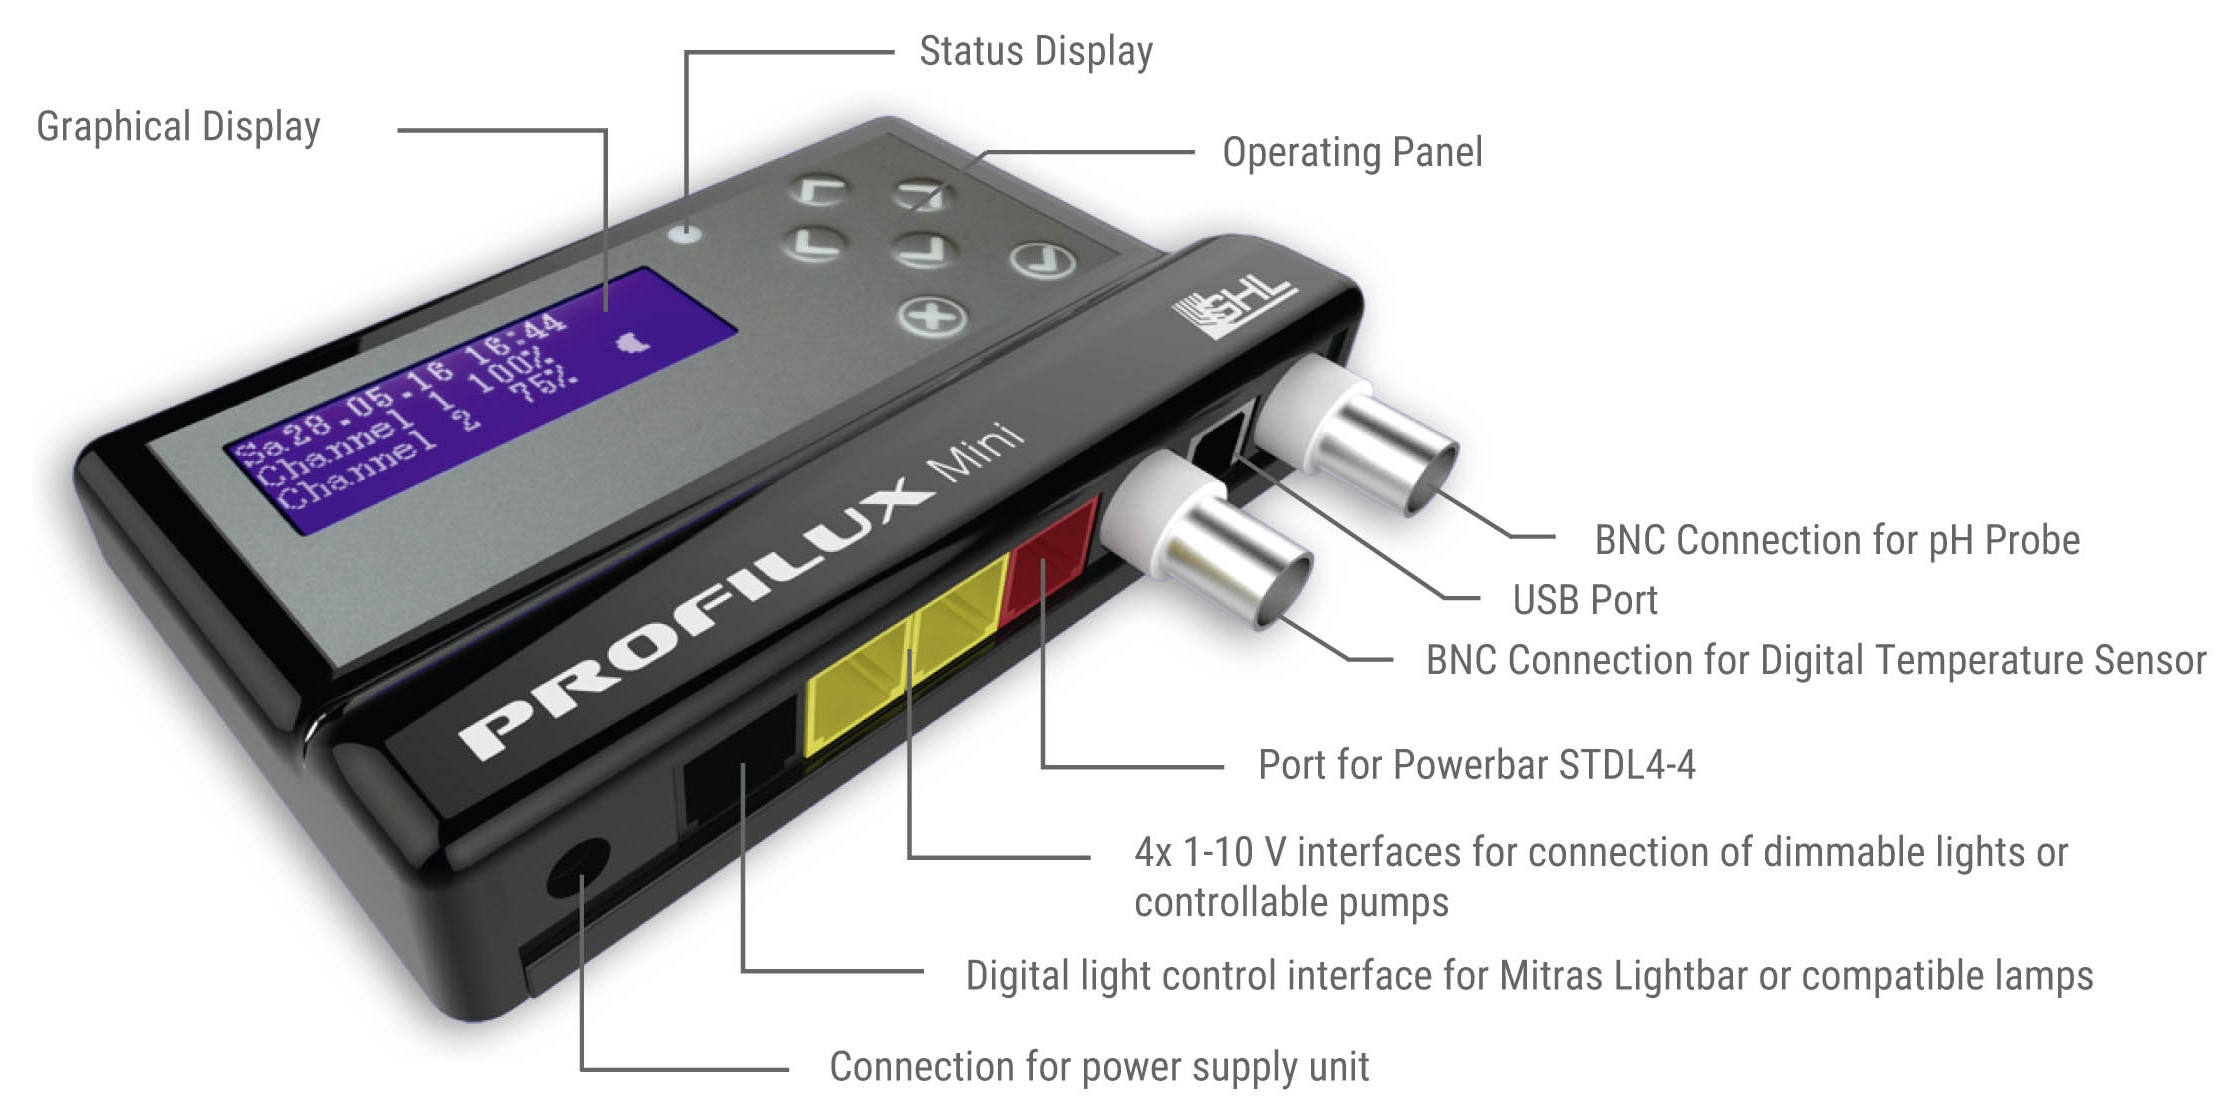
\includegraphics[width=0.9\textwidth]{obrazky/trh/GHL-ProfiLux-Mini.jpg}
                \caption{GHL ProfiLux Mini, nejmenší dostupný kontroler této firmy. Převzato z~\cite{ghl-profilux}.}
                \label{fig:obrazky-trh-GHL-ProfiLux-Mini-jpg}
            \end{figure}
            
        \subsubsection{Neptune Systems -- Apex}
            Systém Apex je nepochybně další ze světových leaderů v této oblasti. Opět je k dispozici několik variant systému podle požadavků a finančních možností uživatele a systém je také velmi modulární. Stejně jako firma GHL, i Neptune Systems je na trhu více než 20 let a jedná se tedy o léty ověřenou značku. Architektura systému je podobná a kromě samotného kontroleru je opět v nabídce celá řada kompatibilních periferií. Dle uživatelských recenzí je konfigurace systému oproti GHL výrazně jednodušší a není nutná znalost programování, navíc systém už od výroby obsahuje přednastavené nejčastější scénáře použití.

            \begin{figure}[h!]
                \centering
                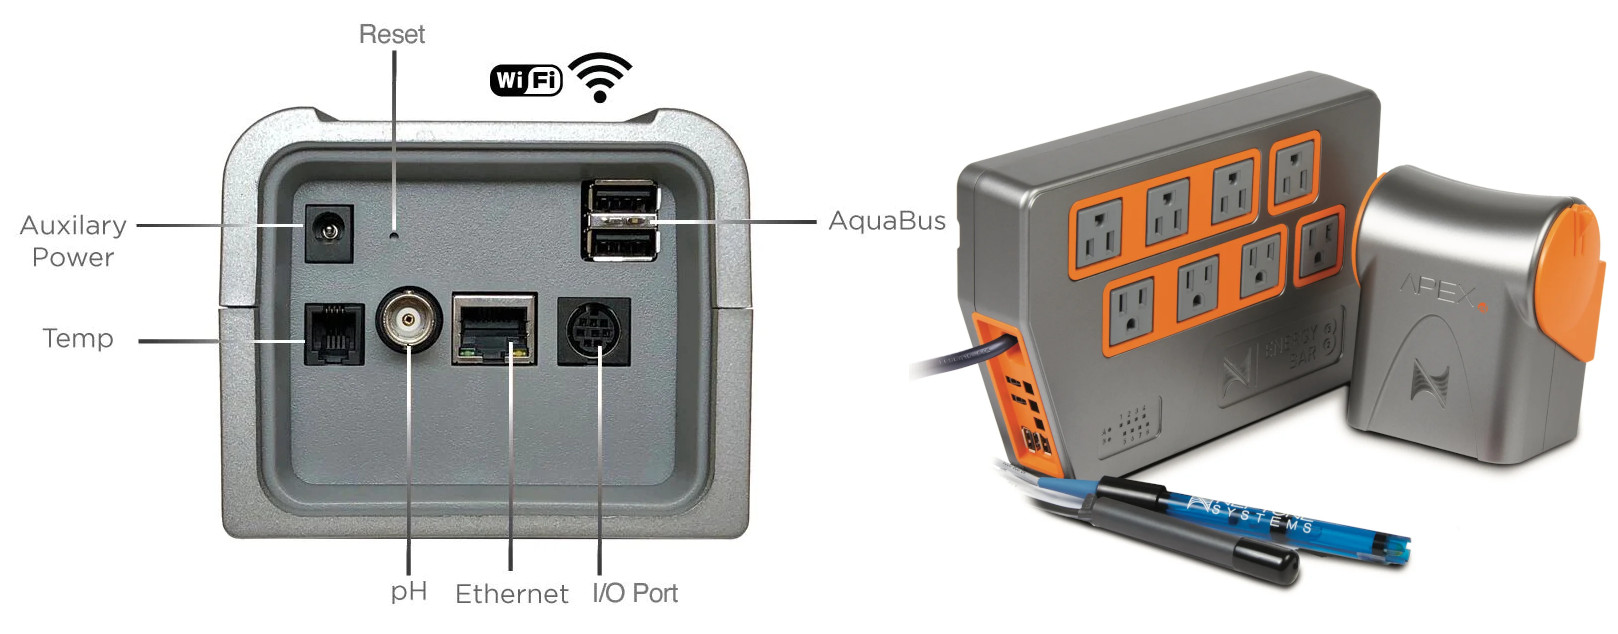
\includegraphics[width=0.8\textwidth]{obrazky/trh/apex-el.jpg}
                \caption{Neptune Systems Apex EL, základní set. Převzato z~\cite{eshop-neptune-systems-apex}.}
                \label{fig:obrazky-trh-apex-el}
            \end{figure}
            
            Cena opět závisí na množství zakoupených modulů, základní set s podobnou výbavou jako u GHL je k dispozici přibližně od \qty{12000}{Kč}~\cite{neptune-systems-why-apex,eshop-neptune-systems-apex}.

        \subsubsection{CoralVue -- HYDROS}
            Firma CoralVue se svým systémem HYDROS je na trhu oproti svým konkurentům relativně krátce, přibližně 3 roky, svým originálním přístupem a cenově dostupným řešením si ale své zákazníky našla rychle. Systém je svou architekturou ještě více modulární než jeho konkurenti, umožňuje v rámci jedné aplikace spojit i více kontrolerů, které mezi sebou komunikují. Dokonce v případě poruchy hlavního kontroleru dokáže jeho roli převzít jiný připojený kontroler a systém tak zůstane dále v provozu. 
            
            Kromě bezdrátově řízeného modulu se čtyřmi síťovými zásuvkami nově firma nabízí také modul, který krom zásuvek obsahuje i vlastní kontroler (Control XP8, viz obr.~\ref{fig:obrazky-hydros-control}), může tak fungovat zcela samostatně, stále však umožňuje také drátové spojení s dalšími kontrolery nebo bezdrátové připojení k dalším zásuvkám. Toto může sloužit jako jednoduché univerzální řešení pro menší akvária s možností budoucího rozšíření. 

            \begin{figure}[h!]
                \centering
                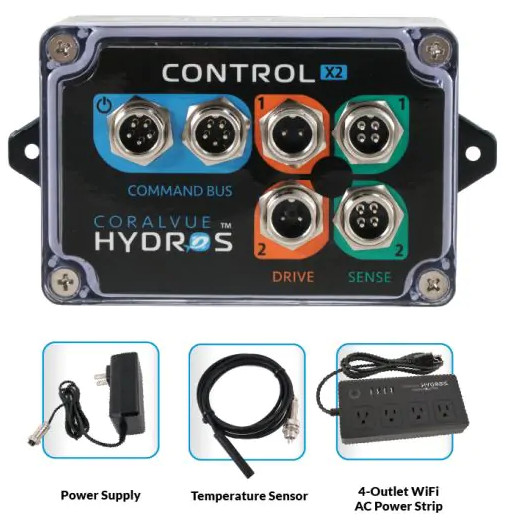
\includegraphics[width=\textwidth]{obrazky/trh/hydros-x2-starter-pack.jpg}
                \caption{CoralVue HYDROS Control X2 Starter pack. Převzato z~\cite{eshop-coralvue-hydros}.}
                \label{fig:obrazky-trh-hydros-x2-starter-pack-jpg}
            \end{figure}
            
            Základní minimální sada je dostupná již od přibližně \qty{4500}{Kč}, aby byla ale výbava stejná jako u výše zmíněných konkurentů je potřeba dokoupit ještě pH sondu za přibližně \qty{800}{Kč}~\cite{coralvuehydros,eshop-coralvue-hydros}.
            
        \subsubsection{Seneye}
            Společnost Seneye nenabízí komplexní řešení pro automatizaci, ale i přesto jsou její produkty zajímavé a pro mnoho akvaristů mohou být skutečně užitečné. Místo pokročilého ovládání akvarijní techniky se výrobky zaměřují pouze na monitorování parametrů vody (popř. dalších veličin), důraz je kladen na maximální jednoduchost použití. Vnitřním sladkovodním akváriím je věnována řada Seneye Home a veškeré monitorování je zajištěno jedním malým zařízením, které uživatel přímo ponoří do vody a pomocí kabelu připojí k počítači ze kterého se zařízení napájí a zároveň do něj odesílá data. Alternativně lze přikoupit také krabičku, která slouží jako webserver, do ní se zařízení připojí namísto počítače a data jsou rovnou zálohována do cloudu, odkud jsou uživateli dostupná v mobilní aplikaci.

            Zařízení monitoruje teplotu, pH, úroveň škodlivého amoniaku, osvětlení a hladinu vody. Umožňuje také odesílat oznámení při překročení nastavené meze některého z parametrů.

            \begin{figure}[h!]
                \centering
                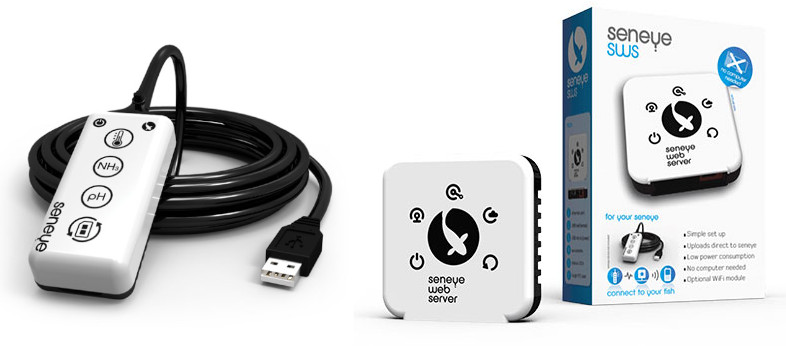
\includegraphics[width=0.8\textwidth]{obrazky/trh/seneye-home.jpg}
                \caption{Seneye Home a Seneye Web Server, převzato z~\cite{seneye-home}.}
                \label{fig:obrazky-trh-seneye-home-jpg}
            \end{figure}

            Cena samotného monitorovacího zařízení je přibližně \qty{3000}{Kč} a podobná je také cena zmíněného webserveru, pro automatické monitorování se zálohou na cloud je tedy potřeba počítat s investicí okolo \qty{6000}{Kč}~\cite{seneye-home}.
            


        